%!TEX encoding = UTF-8 Unicode
% !TeX spellcheck = en_GB
%%%%%%%%%%%%%%%%%%%%%%%%%%%%%%%%%%%%%%
\chapter{ Prospects for Higgs pair production at the FCC }\label{app:fcc}
%%%%%%%%%%%%%%%%%%%%%%%%%%%%%%%%%%%%%%
\section{Orthogonal Projectors in $gg \to ZH$}
 With the caveat of using the 14 TeV $K$-factors for the 100 TeV cross-section scaling, as the 100 TeV $K$-factors were not available for all processes. I should note that we have explicitly checked that at least within the SM, for Higgs pair production via gluon fusion the difference is of $\mathcal{O}(1\%)$~\cite{Maltoni:2014eza} and hence small.
 
 
 \begin{table}[]
 	\centering
 	{\footnotesize
 		
 		\begin{tabular}{ll|rrrrr|r}
 			\multirow{7}{*}{\rb{\bf Actual no. of events\hspace{0.45cm}}} & \multicolumn{7}{c}{\bf Predicted no. of events at FCC-hh}\\
 			\cmidrule[\heavyrulewidth]{2-8}
 			& Channel & $\hhtri$ & $\hhtri$ &  $\hhbox$&      $\QQh$ & $\bbaa$ &   total \\
 			\cline{2-8}
 			&$\hhtri$       &  	3,579& 1,303&	2,372&	4,697&	337&	12,288 \\
 			&$\hhint$       &  13,602& 7,300&	17,075&	24,716&	1523&	64,216 \\
 			&$\hhbox$       &  14,534&	11,416&	35,988&	415,26& 1,996&	105,460 \\
 			&$\QQh$         & 29,611&	12,355&	23,279&	1,238,266&	214,564&	1,518,075 \\
 			&$\bbaa$        &  45,574&	22,290&	26,213&	150,935&	227,142&	24,317,657 \\
 			\cline{2-8}
 			&$\mathcal{Z}_j$&   	10.95&	31.22&	111.1&	737.7&	4,743&	 \\
 			\cmidrule[\heavyrulewidth]{2-8}
 		\end{tabular}
 	}
 	\caption{\it Trained BDT classification (confusion matrix) of the five channel used to extract constraints on $C_\phi$ (or $\kappa_\lambda$) at FCC-hh with 30 $\iab$ luminosity, assuming SM signal injection. The right-most column gives the total number of events expected in each channel in the SM and the bottom-most row gives the signal significance.}
 	\label{tab:FCC-hh-confusion-CH}
 \end{table}
 The projected bounds on these operators at FCC-hh with 30$\inab$ of data using our framework are
\begin{equation}
	\begin{split}
		C_{u\phi}^{MV} \left(\kappa_u^{MV}\right) = [-0.012, 0.011] \;([-57.8, 54.7])\,,\\
		C_{d\phi}^{MV} (\kappa_d^{MV}) = [-0.012, 0.012] \;([-26.3, 28.4])\,.
	\end{split}
\end{equation}
\begin{table}[]
	\centering
	{\footnotesize
		\begin{tabular}{cccc||ccc}
			\toprule
			Operators &  $C_{u\phi}$&   $C_{d\phi}$&   $C_{\phi}$&    $\kappa_{u}$&   $\kappa_{d}$&   $\kappa_\lambda$\\
			\multicolumn{7}{c}{FCC-hh 100 TeV 30$\inab$}\\
			\midrule
			$\mathcal O_{\phi}$ &--   & --            &[-0.066, 0.064] &--  & -- &[0.97, 1.03]\\
			$\mathcal O_{u\phi}$&[-0.012, 0.011]   & --            &-- &[-57.8, 54.7]  & -- &--\\
			$\mathcal O_{d\phi}$&--   & [-0.012, 0.011]            &-- &--  & [-26.3, 28.4] &--\\
			$\mathcal O_{u\phi}$ \& $\mathcal O_{\phi}$ &[-0.010, 0.011]  & --            &[-0.091, 0.042] &[-52, 49] & -- &[0.98, 1.04]\\
			$\mathcal O_{d\phi}$ \& $\mathcal O_{\phi}$ & --             &[-0.010, 0.012]  &[-0.092, 0.041]& -- &[-24, 26] &[0.98, 1.04]\\
			$\mathcal O_{u\phi}$ \& $\mathcal O_{d\phi}$&[-0.008, 0.009]&[-0.008, 0.009]& --            &[-42, 39] &[-19,19] & -- \\
			All                                   &[-0.009, 0.010]&[-0.009, 0.010]& [-0.105 0.023]&[-47, 44] &[-21, 21] & [0.99, 1.05] \\
			\bottomrule
		\end{tabular}
	}
	\caption{\it The 1$\sigma$ bounds on $C_{u\phi}$, $C_{d\phi}$ and $C_\phi$ from one-, two- and three-parameter fits for HL-LHC with 6$\inab$ of data and FCC-hh with 30$\inab$ of data. The corresponding bounds on the rescaling of the effective couplings, $\kappa_u$, $\kappa_d$ and $\kappa_\lambda$ are presented on the right side of the table.}
	\label{tab:twoparambounds}
\end{table}
These projected bounds for FCC-hh are an order of magnitude better than those for HL-LHC. In addition, the bounds on $C_{u\phi}$ and $C_{d\phi}$ are numerically the same displaying a much greater improvement in the bounds on $C_{d\phi}$ than on $C_{u\phi}$ at the higher energy collider. 
\begin{figure}[t!]
	\centering
	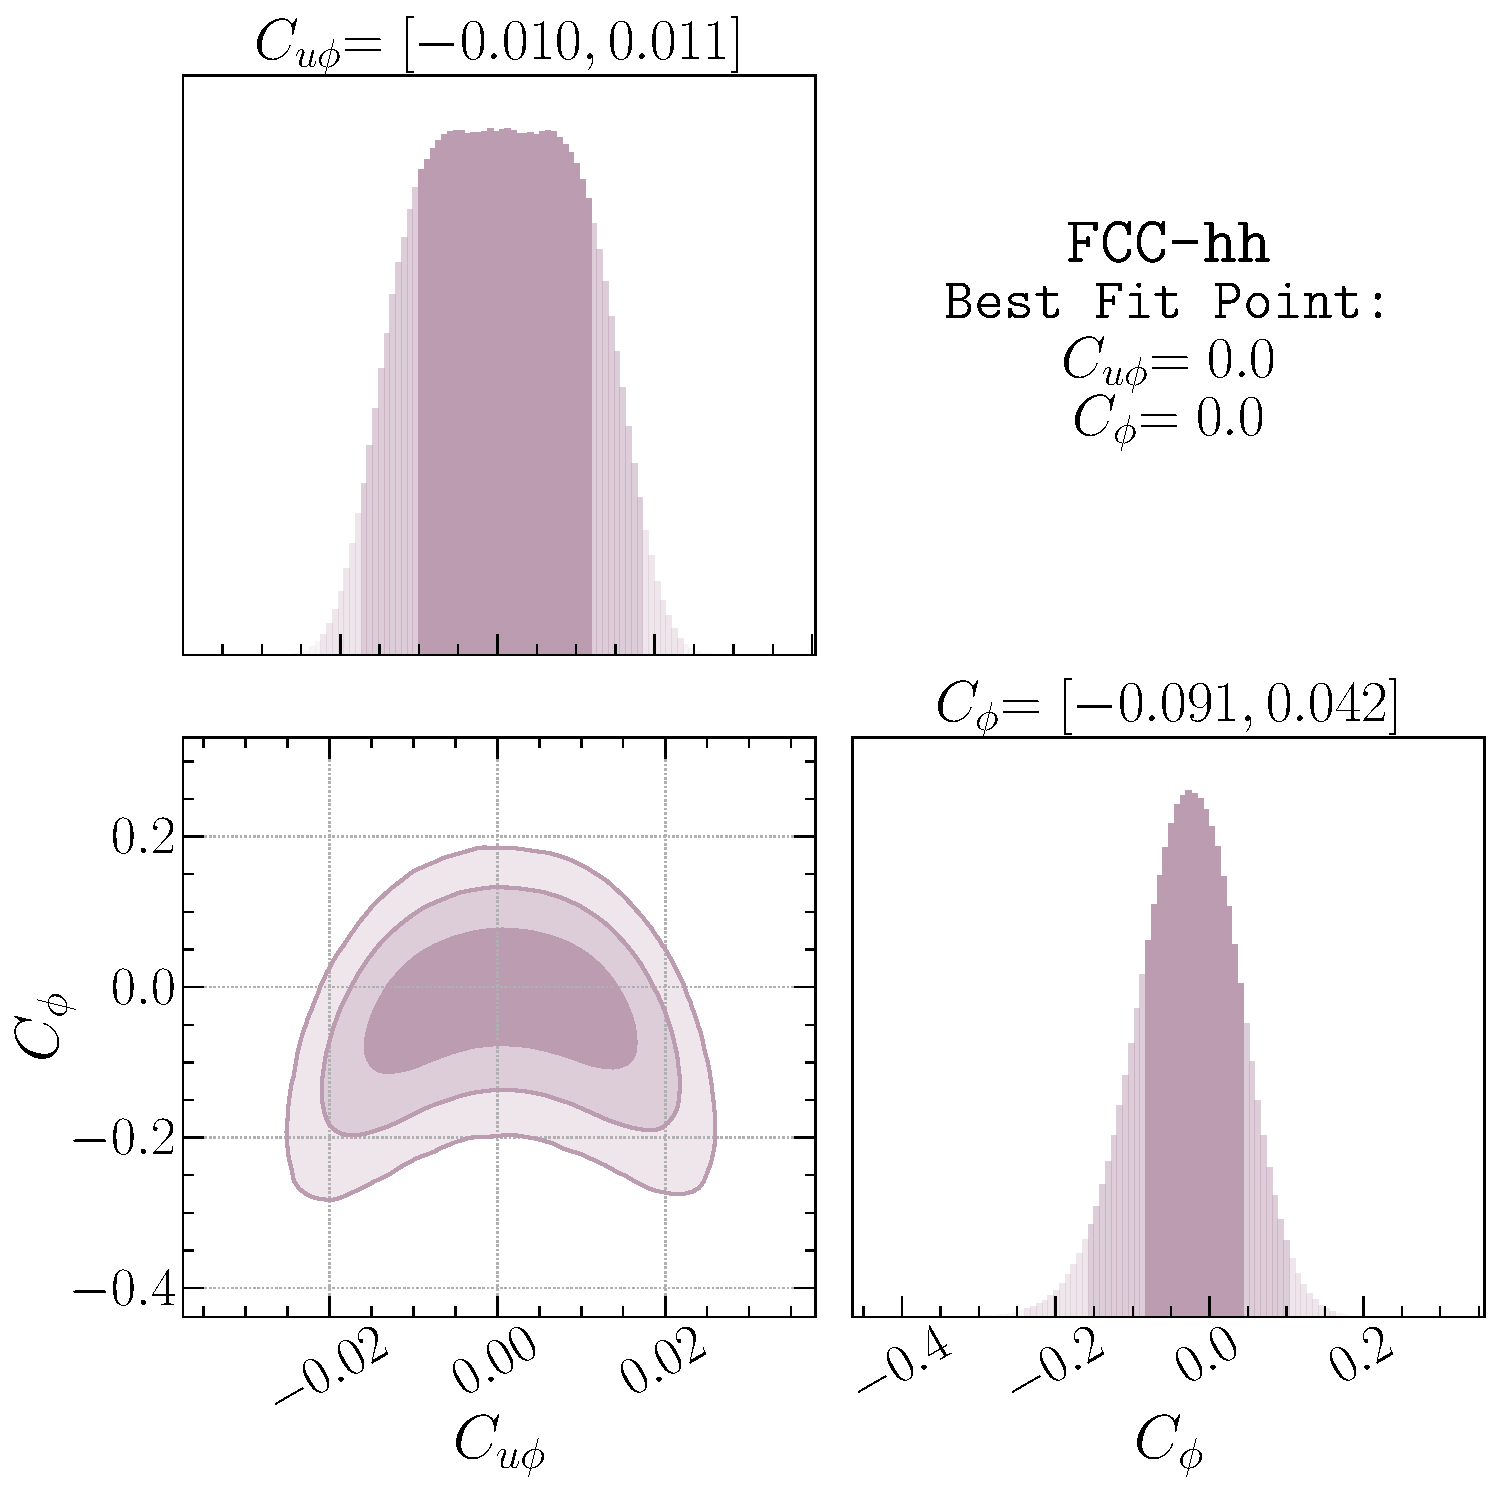
\includegraphics[width=0.47\linewidth]{fig/kappa_u-kappa_l-FCC-hh.pdf}
	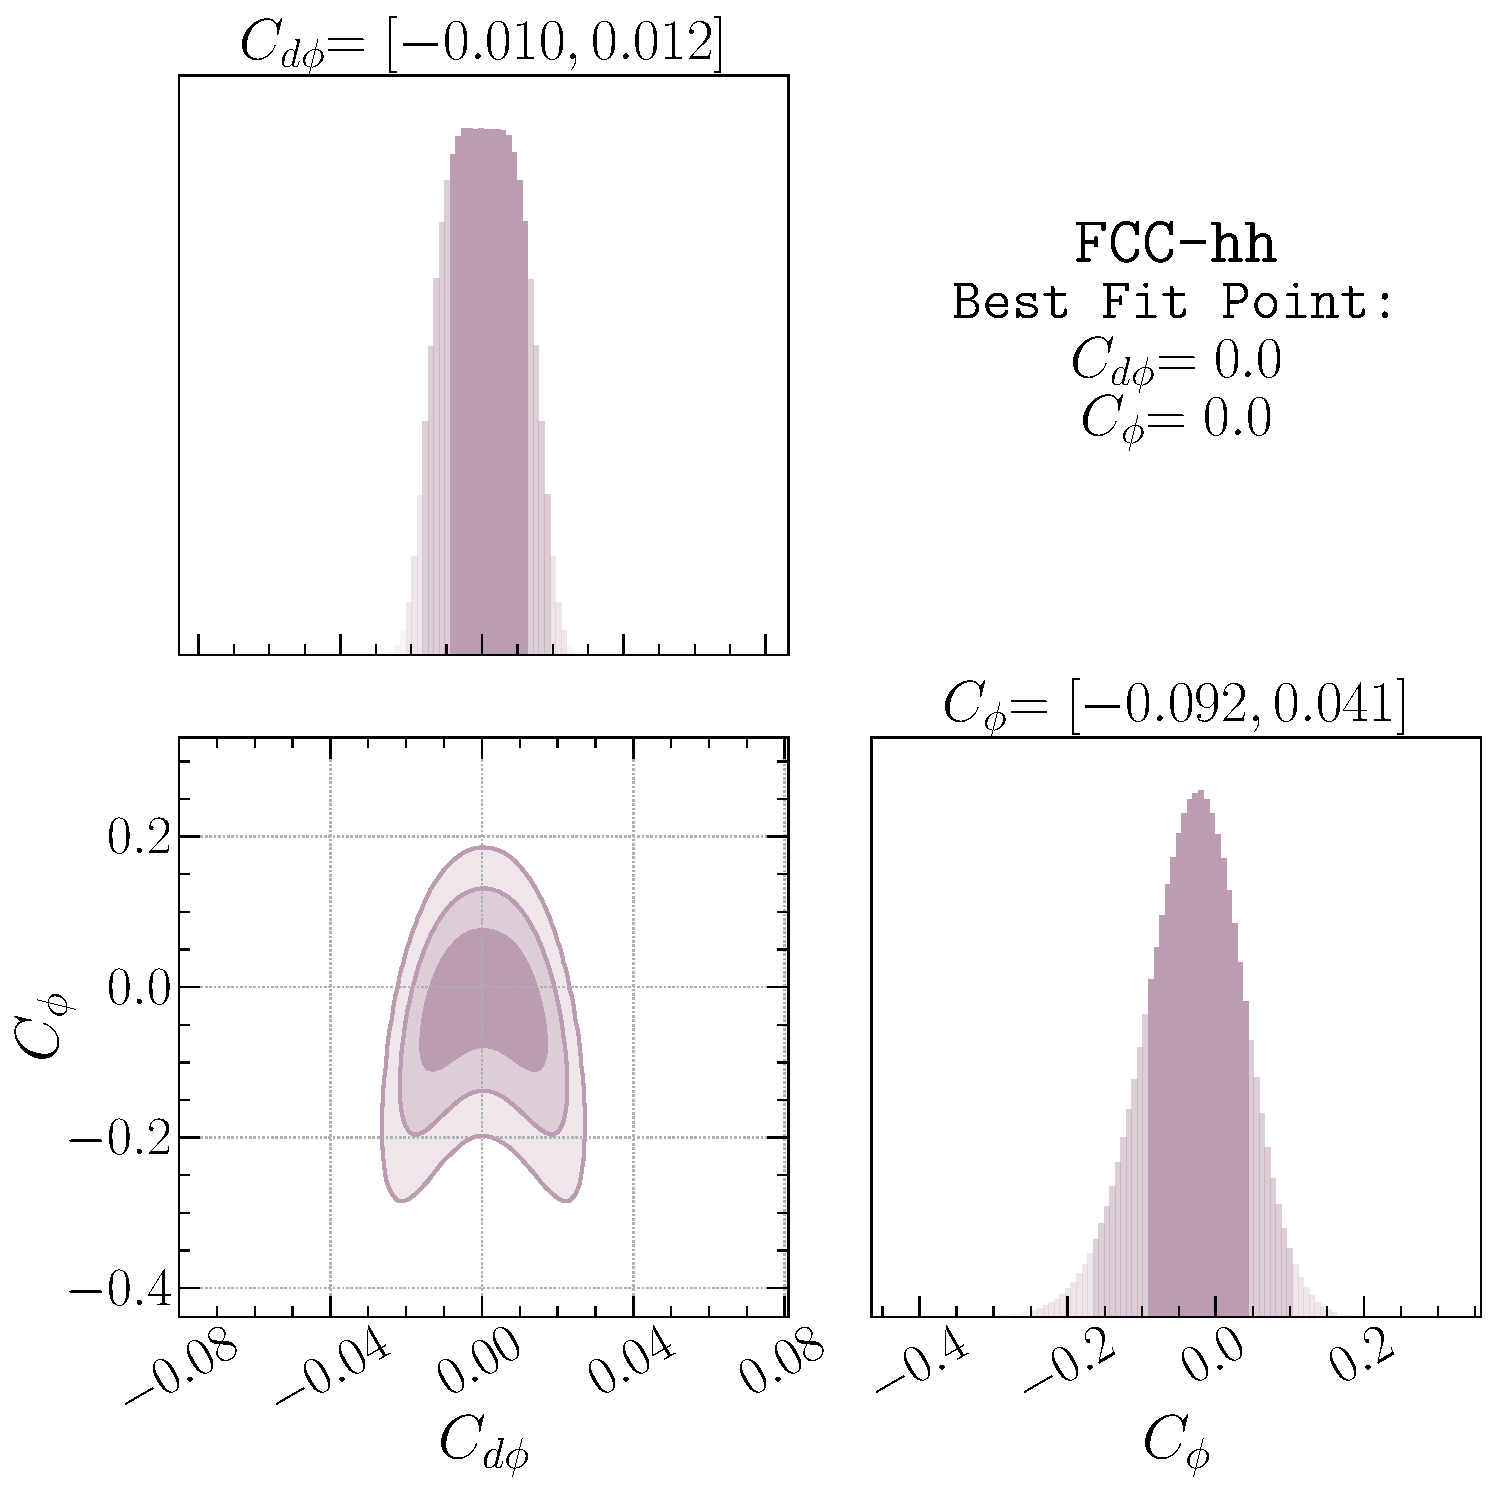
\includegraphics[width=0.47\linewidth]{fig/kappa_d-kappa_l-FCC-hh.pdf}
	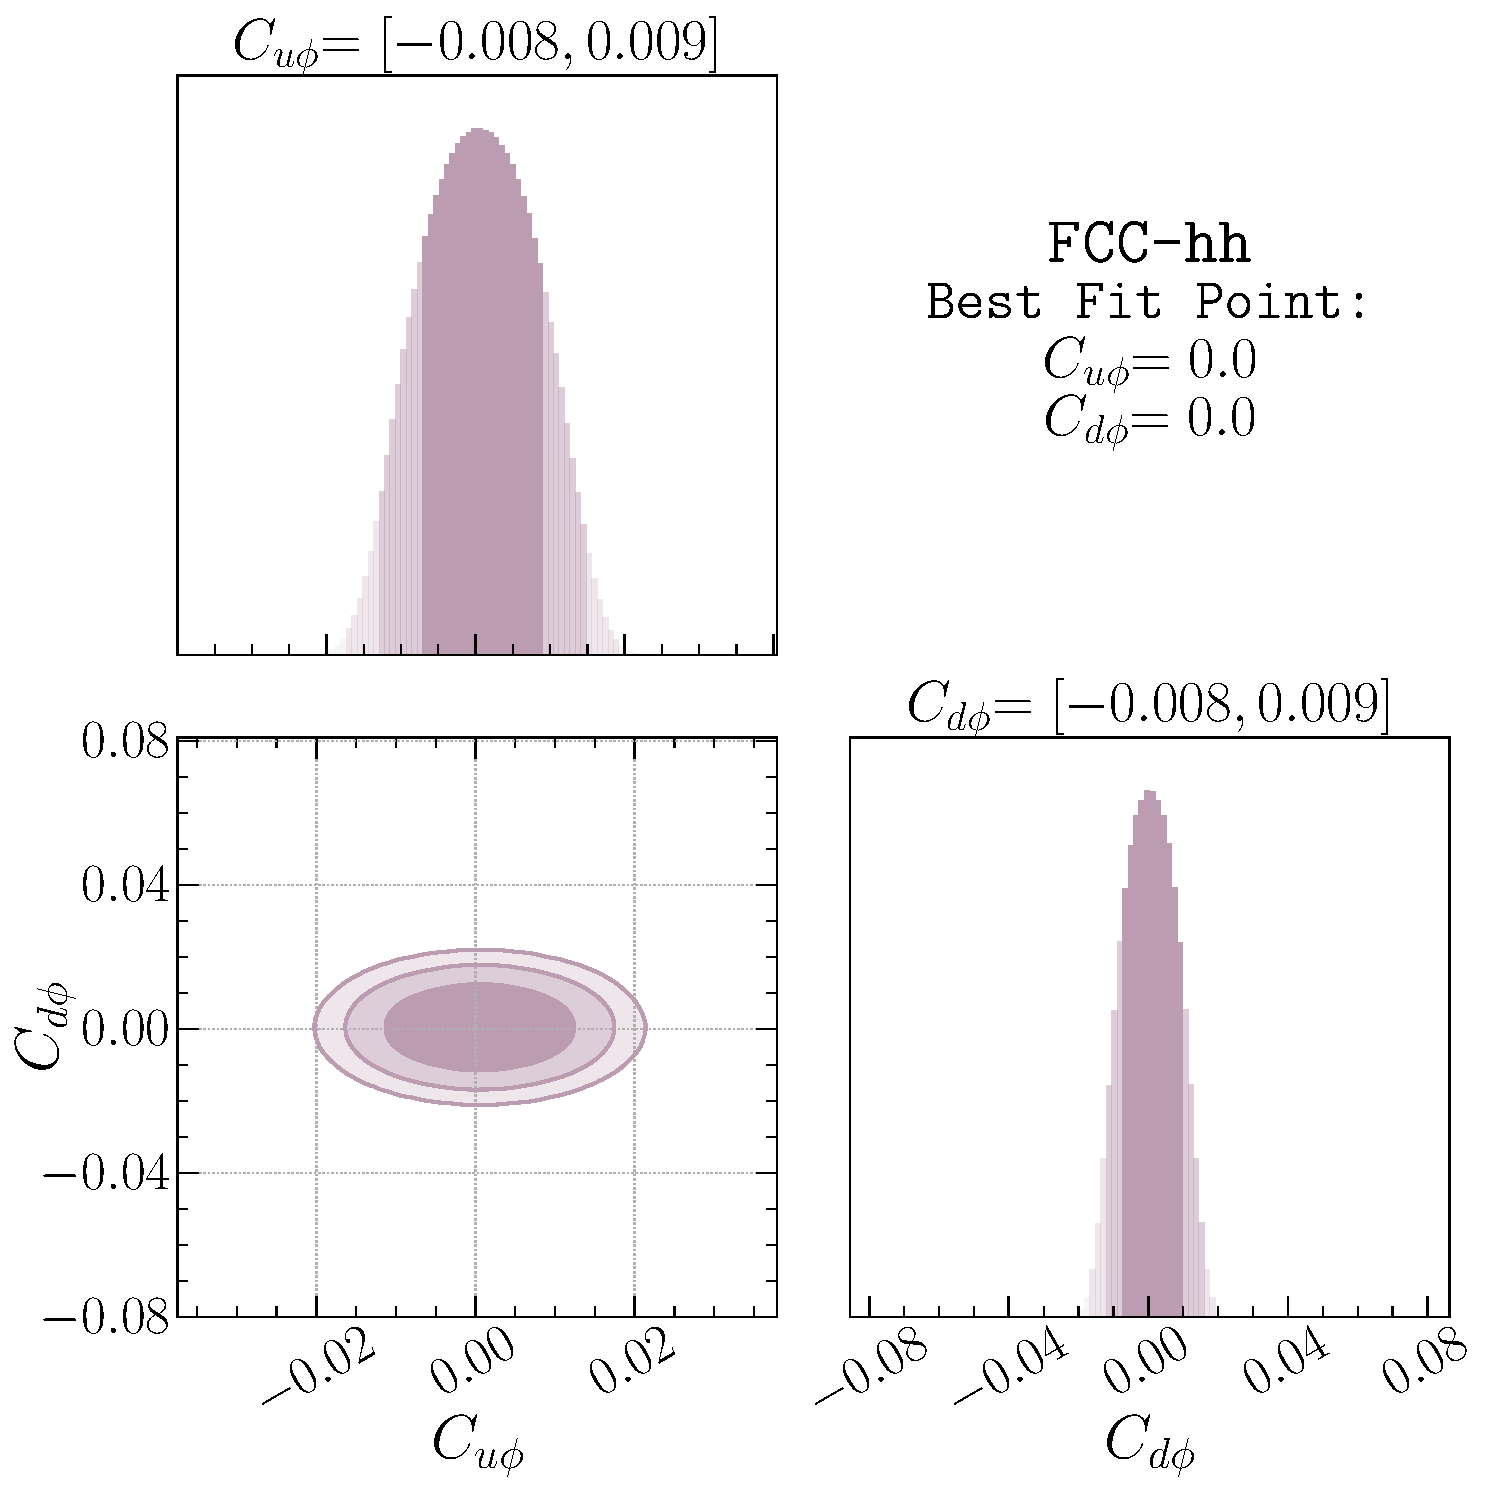
\includegraphics[width=0.47\linewidth]{fig/kappa_u-kappa_d-FCC-hh.pdf}
	\caption{\it Constraints on pairs of Wilson coefficients for $C_\phi$, $C_{u\phi}$ and $C_{d\phi}$, The panels of the left are for HL-LHC with 6 $\iab$ of luminosity and the ones on the right are for FCC-hh with 30 $\iab$ of luminosity.}
	\label{fig:constraint2d}
\end{figure}
\FloatBarrier

\begin{figure}[t!]
	\centering
	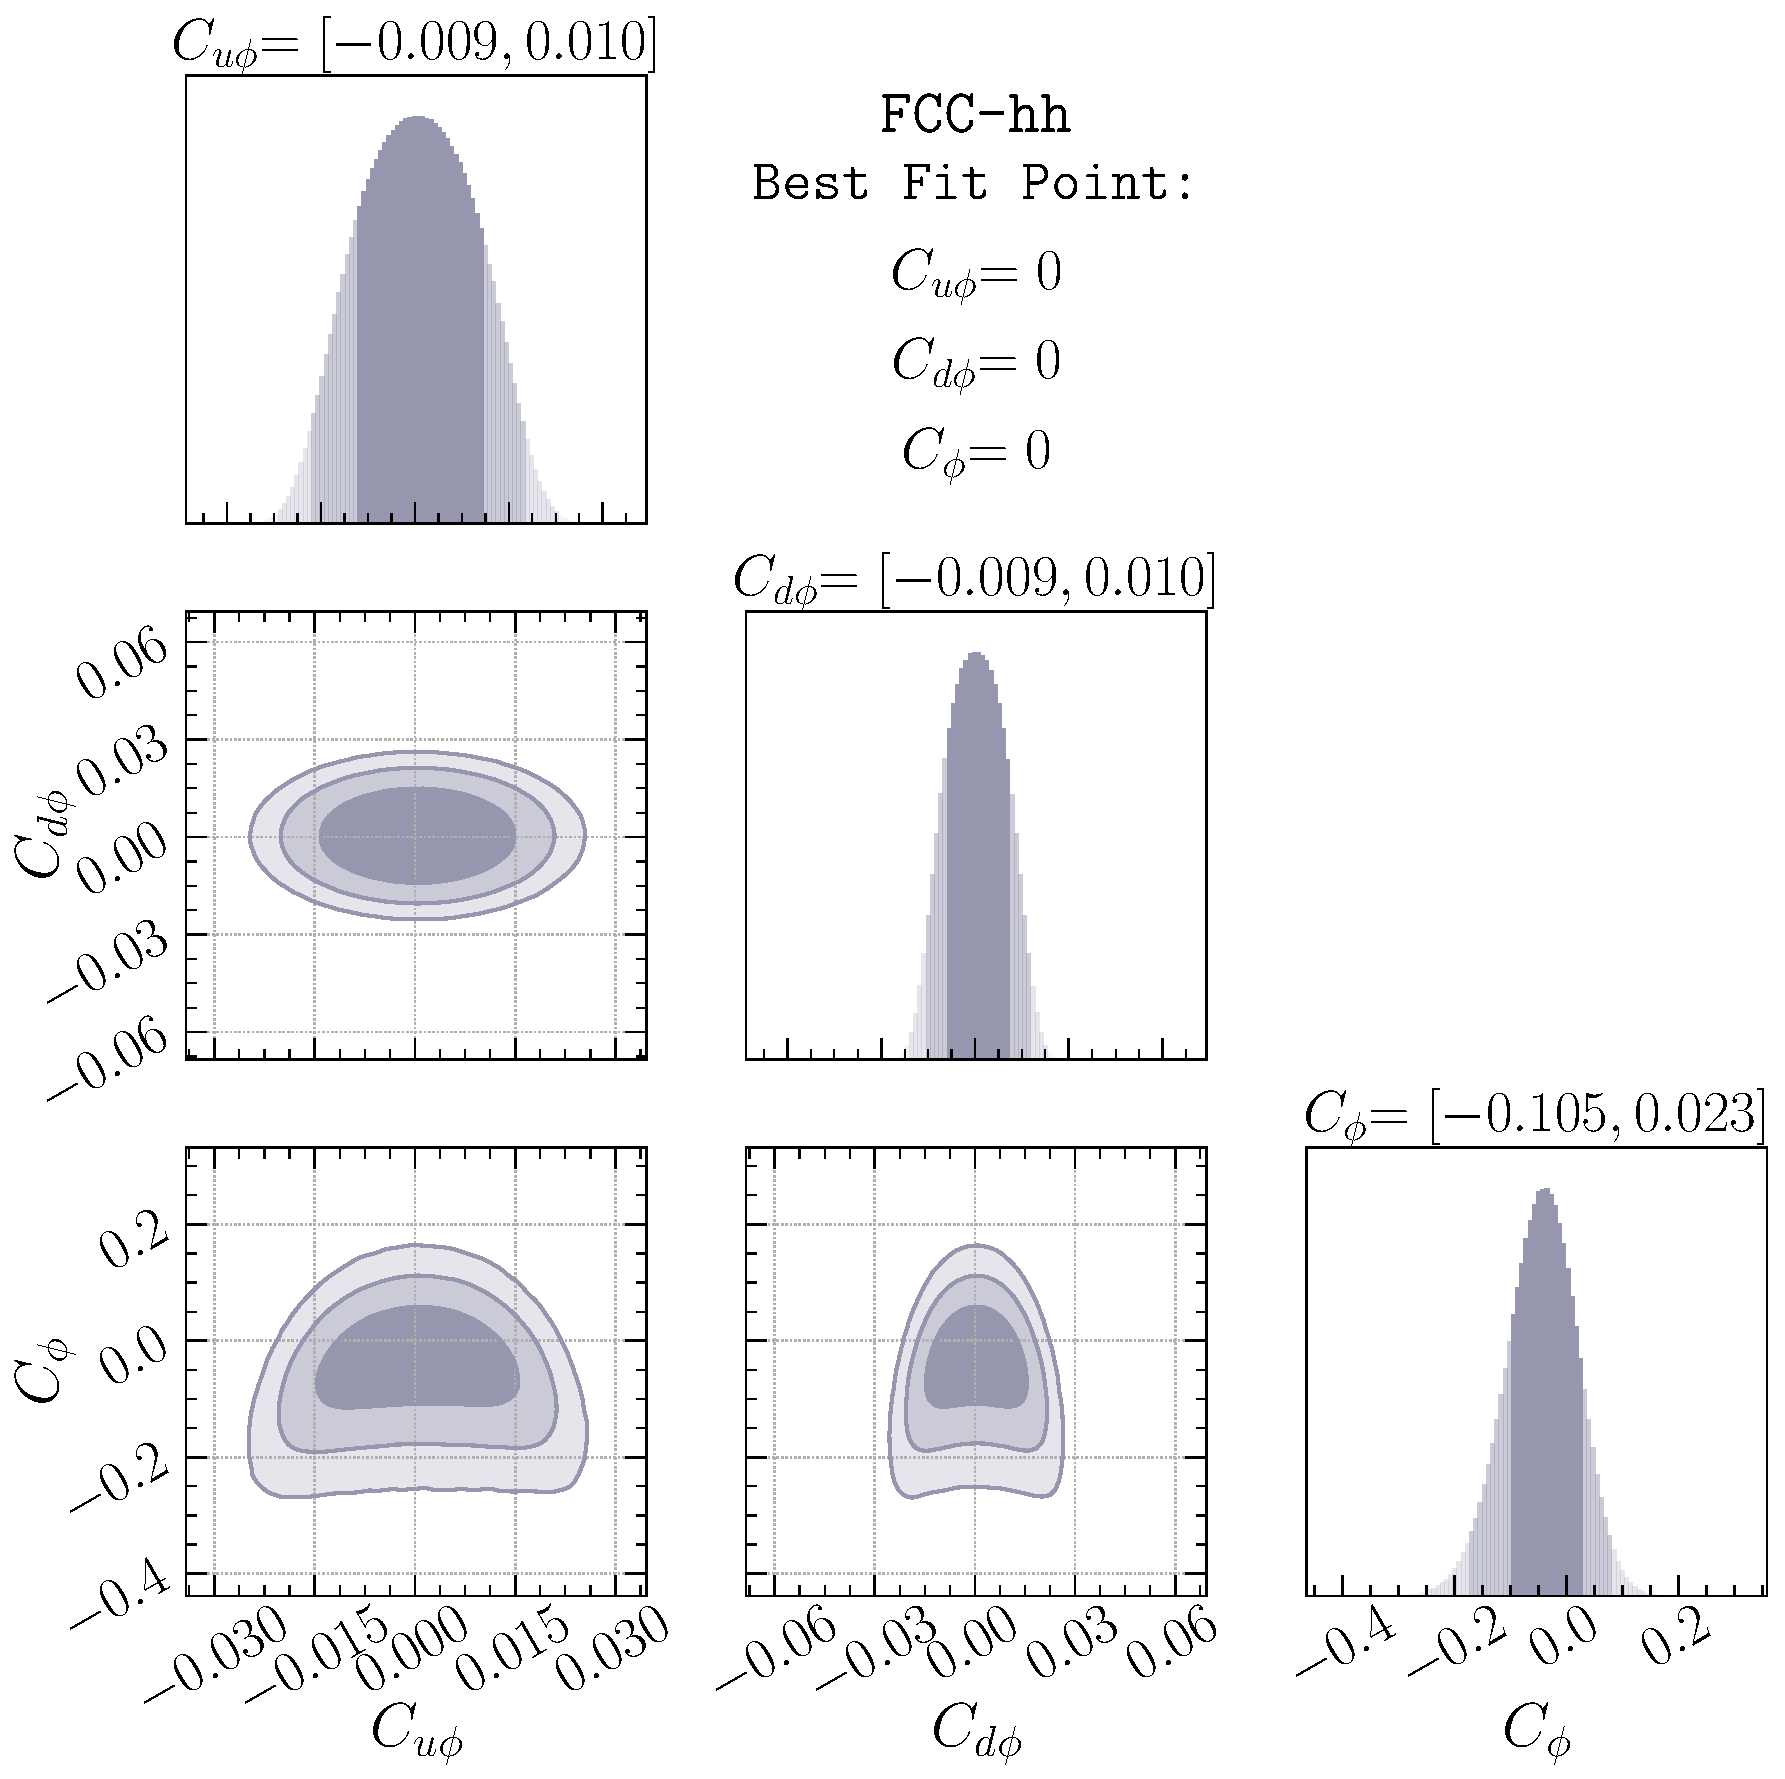
\includegraphics[width =0.47\linewidth]{fig/kappa_u-kappa_d-kappa_l-FCC-hh.pdf}
	\caption{\it Three parameter fits with $C_{u\phi}$, $C_{d\phi}$ and $C_\phi$, 6$\inab$ of luminosity at 14 TeV for HL-LHC (left panel) and 30$\inab$ of luminosity at 100 TeV for FCC-hh (right panel).}
	\label{fig:constraint3d}
\end{figure}
